
%%%%%%%%%%%%%%%%%%%%%%%%%%%%%%%%%%%%%%%%%%%%%%%%%%%%%%%%%%%%%%%%%%%%%%%%%%%%%%
% Copyright (c) 2003-2018 by The University of Queensland
% http://www.uq.edu.au
%
% Primary Business: Queensland, Australia
% Licensed under the Apache License, version 2.0
% http://www.apache.org/licenses/LICENSE-2.0
%
% Development until 2012 by Earth Systems Science Computational Center (ESSCC)
% Development 2012-2013 by School of Earth Sciences
% Development from 2014 by Centre for Geoscience Computing (GeoComp)
%
%%%%%%%%%%%%%%%%%%%%%%%%%%%%%%%%%%%%%%%%%%%%%%%%%%%%%%%%%%%%%%%%%%%%%%%%%%%%%%

\chapter{The \linearPDEs Module}

\section{Linear Partial Differential Equations}
\label{SEC LinearPDE}

The \LinearPDE class is used to define a general linear, steady, second order
PDE for an unknown function $u$ on a given $\Omega$ defined through a \Domain object.
In the following $\Gamma$ denotes the boundary of the domain $\Omega$ and $n$
denotes the outer normal field on $\Gamma$.

For a single PDE with a solution that has a single component the linear PDE is
defined in the following form \footnote{This PDE system can be written in the equivalent form, \begin{align*} \centering \, -\nabla \cdot \left( \textbf{A} \nabla u \right) - \nabla \cdot \left( \textbf{B} \, u \right) + \textbf{C} \cdot \nabla u + \textbf{D} \, u + \sum_p \delta(p) u(p) &= - \nabla \cdot \textbf{X} + \textbf{Y} + \sum_p \delta(p), \\
	\hat{\textbf{n}} \cdot \left( \textbf{A} \nabla u + \textbf{B} \, u \right) + \textbf{d} \, u &= \hat{\textbf{n}} \cdot \textbf{X} + \textbf{y}, 
\end{align*} where bold font denotes a data object and $\hat{\textbf{n}}$ denotes a unit vector normal.  The weak form for this is
\begin{equation*}\int_{\Omega} (\nabla v)\cdot \left( \textbf{A} \nabla u \right) +( \nabla v) \cdot \left( \textbf{B} \, u \right) + v\textbf{C} \cdot \nabla u + \textbf{D} \,v u + \sum_p \delta(p) u(p)v \;d\Omega = \int_{\Omega}(\nabla v) \cdot \textbf{X} + \textbf{Y}v + \sum_p \delta(p)v\; d\Omega.
\end{equation*}
}
\begin{equation}\label{LINEARPDE.SINGLE.1}
-(A_{jl} u_{,l})_{,j}-(B_{j} u)_{,j}+C_{l} u_{,l}+D u + \sum_p d^{dirac}(p) \; u(p) =-X_{j,j}+Y + \sum_p y^{dirac}(p)  \; .
\end{equation}
$u_{,j}$ denotes the derivative of $u$ with respect to the $j$-th spatial direction.
Einstein's summation convention, i.e. summation over indexes appearing twice
in a term of a sum, is used in this chapter. $y^{dirac}(p)$ represent a nodal source term 
at point $p$, cf. $y^{dirac}(p) $ and similar $d^{dirac}(p)$ define Dirac delta-function 
terms. 
The coefficients $A$, $B$, $C$, $D$, $X$ and $Y$ have to be specified through
\Data objects in the \Function on the PDE or objects that can be converted
into such \Data objects. $d^{dirac}$
$A$ is a \RankTwo, $B$, $C$ and $X$ are each a \RankOne and $D$ and $Y$ are
scalars. $y^{dirac}$ and $d^{dirac}$ are each scalars in the \DiracDeltaFunctions. 
The following natural boundary conditions are considered\index{boundary condition!natural} on $\Gamma$: 
\begin{equation}\label{LINEARPDE.SINGLE.2}
n_{j}(A_{jl} u_{,l}+B_{j} u)+d u=n_{j}X_{j} + y  \;.
\end{equation}
Notice that the coefficients $A$, $B$ and $X$ are defined in the PDE.
The coefficients $d$ and $y$ are each a \Scalar in the \FunctionOnBoundary.
Constraints\index{constraint} for the solution prescribe the value of the
solution at certain locations in the domain. They have the form
\begin{equation}\label{LINEARPDE.SINGLE.3}
u=r \mbox{ where } q>0
\end{equation}
$r$ and $q$ are each a \Scalar where $q$ is the characteristic function\index{characteristic function}
defining where the constraint is applied.
The constraints defined by \eqn{LINEARPDE.SINGLE.3} override any other
condition set by \eqn{LINEARPDE.SINGLE.1} or \eqn{LINEARPDE.SINGLE.2}.

For a system of PDEs and a solution with several components the PDE has the form
\begin{equation}\label{LINEARPDE.SYSTEM.1}
-(A_{ijkl} u_{k,l})_{,j}-(B_{ijk} u_{k})_{,j}+C_{ikl} u_{k,l}+D_{ik} u_{k}+
 \sum_p d^{dirac}_{ik}(p) \;  u_i(p)
 =-X_{ij,j}+Y_{i} +\sum_p \; y^{dirac}_i(p)   \; .
\end{equation}
$A$ is a \RankFour, $B$ and $C$ are each a \RankThree, $D$, $d^{dirac}$ and $X$ are each a \RankTwo and $Y$ and $y^{dirac}$ is a \RankOne.
The natural boundary conditions\index{boundary condition!natural} take the form:
\begin{equation}\label{LINEARPDE.SYSTEM.2}
n_{j}(A_{ijkl} u_{k,l}+B_{ijk} u_{k})+d_{ik} u_{k}=n_{j}X_{ij}+y_{i}  \;.
\end{equation}
The coefficient $d$ is a \RankTwo and $y$ is a \RankOne both in the
\FunctionOnBoundary. Constraints\index{constraint} take the form
\begin{equation}\label{LINEARPDE.SYSTEM.3}
u_{i}=r_{i} \mbox{ where } q_{i}>0
\end{equation}
$r$ and $q$ are each a \RankOne. Notice that not necessarily all components
must have a constraint at all locations.  An example for a system of PDEs is shown in the elastic deformation example in section \ref{ELASTIC CHAP}

\LinearPDE also supports solution discontinuities\index{discontinuity} over a
contact region $\Gamma^{contact}$ in the domain $\Omega$.
To specify the conditions across the discontinuity we are using the
generalised flux $J$\footnote{In some applications the definition of flux used
here can be different from the commonly used definition.
For instance, if $T$ is a temperature field the heat flux $q$ is defined as
$q_{,i}=-\kappa T_{,i}$ ($\kappa$ is the diffusivity) which differs from the
definition used here by the sign. This needs to be kept in mind when defining
natural boundary conditions\index{boundary condition!natural}.} which in
the case of a system of PDEs and several components of the solution, is
defined as
\begin{equation}\label{LINEARPDE.SYSTEM.5}
J_{ij}=A_{ijkl}u_{k,l}+B_{ijk}u_{k}-X_{ij}
\end{equation}
For the case of single solution component and single PDE, $J$ is defined as
\begin{equation}\label{LINEARPDE.SINGLE.5}
J_{j}=A_{jl}u_{,l}+B_{j}u_{k}-X_{j}
\end{equation}
In the context of discontinuities\index{discontinuity} $n$ denotes the normal
on the discontinuity pointing from side 0 towards side 1.
For a system of PDEs the contact condition takes the form
\begin{equation}\label{LINEARPDE.SYSTEM.6}
n_{j} J^{0}_{ij}=n_{j} J^{1}_{ij}=y^{contact}_{i} - d^{contact}_{ik} [u]_{k} \; .
\end{equation}
where $J^{0}$ and $J^{1}$ are the fluxes on side $0$ and side $1$ of the
discontinuity $\Gamma^{contact}$, respectively. $[u]$, which is the difference
of the solution at side 1 and at side 0, denotes the jump of $u$ across $\Gamma^{contact}$.
The coefficient $d^{contact}$ is a \RankTwo and $y^{contact}$ is a
\RankOne both in the \FunctionOnContactZero or \FunctionOnContactOne.
In the case of a single PDE and a single component solution the contact
condition takes the form
\begin{equation}\label{LINEARPDE.SINGLE.6}
n_{j} J^{0}_{j}=n_{j} J^{1}_{j}=y^{contact} - d^{contact}[u]
\end{equation}
In this case the coefficient $d^{contact}$ and $y^{contact}$ are each
\Scalars both in either\\
the \FunctionOnContactZero or the \FunctionOnContactOne.

The PDE is symmetrical\index{symmetrical} if
\begin{equation}\label{LINEARPDE.SINGLE.4}
A_{jl}=A_{lj} \mbox{ and } B_{j}=C_{j}
\end{equation}
The system of PDEs is symmetrical\index{symmetrical} if
\begin{eqnarray}
\label{LINEARPDE.SYSTEM.4}
A_{ijkl}&=&A_{klij} \\
B_{ijk}&=&C_{kij} \\
D_{ik}&=&D_{ki} \\
d_{ik}&=&d_{ki} \\
d^{contact}_{ik}&=&d^{contact}_{ki}
\end{eqnarray}
Note that in contrast to the scalar case \eqn{LINEARPDE.SINGLE.4} now the
coefficients $D$, $d$ and $d^{contact}$ have to be inspected.

The following example illustrates a typical usage of the \LinearPDE class:
\begin{python}
  from esys.escript import *
  from esys.escript.linearPDEs import LinearPDE
  from esys.finley import Rectangle
  mydomain = Rectangle(l0=1., l1=1., n0=40, n1=20)
  mypde=LinearPDE(mydomain)
  mypde.setSymmetryOn()
  mypde.setValue(A=kappa*kronecker(mydomain), D=1, Y=1)
  u=mypde.getSolution()
\end{python}
We refer to \Chap{CHAP: Tutorial} for more details.

An instance of the \SolverOptions class is attached to the \LinearPDE class
object. It holds options for the solver that may be set before solving the PDE.
In the following example the \method{getSolverOptions} method is used to
access the \SolverOptions object attached to \var{mypde}:
\begin{python}
  from esys.escript import *
  from esys.escript.linearPDEs import LinearPDE, SolverOptions
  from esys.finley import Rectangle
  mydomain = Rectangle(l0=1., l1=1., n0=40, n1=20)
  mypde=LinearPDE(mydomain)
  mypde.setValue(A=kappa*kronecker(mydomain), D=1, Y=1)
  mypde.getSolverOptions().setVerbosityOn()
  mypde.getSolverOptions().setSolverMethod(SolverOptions.PCG)
  mypde.getSolverOptions().setPreconditioner(SolverOptions.AMG)
  mypde.getSolverOptions().setTolerance(1e-8)
  mypde.getSolverOptions().setIterMax(1000)
  u=mypde.getSolution()
\end{python}
In this example, the preconditioned conjugate gradient method \PCG is used
with preconditioner \AMG. The relative tolerance is set to $10^{-8}$ and
the maximum number of iteration steps to $1000$.
After a completed call to \method{getSolution()}, the attached \SolverOptions
object gives access to diagnostic information:
\begin{python}
  u=mypde.getSolution()
  print("Number of iteration steps =", mypde.getDiagnostics("num_iter"))
  print("Total solution time =", mypde.getDiagnostics("time"))
  print("Set-up time =", mypde.getDiagnostics("set_up_time"))
  print("Net time =", mypde.getDiagnostics("net_time"))
  print("Residual norm of returned solution =", 
      mypde.getDiagnostics('residual_norm'))
\end{python}
Typically, a negative value for a diagnostic variable indicates that it is
undefined.  For more details on \SolverOptions and Trilinos see chapter \ref{TRILINOS}.

\subsection{Classes}
%\declaremodule{extension}{esys.escript.linearPDEs} 
%\modulesynopsis{Linear partial differential equation handler}
The module \linearPDEs provides an interface to define and solve linear partial
differential equations within \escript. The module \linearPDEs does not
provide any solver capabilities in itself but hands the PDE over to the PDE
solver library defined through the \Domain of the PDE, e.g. \finley.
The general interface is provided through the \LinearPDE class. The \Poisson
class which is also derived form the \LinearPDE class can be used to define
the Poisson equation\index{Poisson}.

\subsection{\LinearPDE class}
This is the general class to define a linear PDE in \escript.
We list a selection of the most important methods of the class.
For a complete list, see the reference at \ReferenceGuide.

\begin{classdesc}{LinearPDE}{domain,numEquations=0,numSolutions=0}
opens a linear, steady, second order PDE on the \Domain \var{domain}.
The parameters \var{numEquations} and \var{numSolutions} give the number of
equations and the number of solution components.
If \var{numEquations} and \var{numSolutions} are non-positive, then the number
of equations and the number of solutions, respectively, stay undefined until a
coefficient is defined.
\end{classdesc}

\subsubsection{\LinearPDE methods}
\begin{methoddesc}[LinearPDE]{setValue}{
\optional{A}\optional{, B},
\optional{, C}\optional{, D}
\optional{, X}\optional{, Y}
\optional{, d}\optional{, y}
\optional{, d_contact}\optional{, y_contact}
\optional{, d_dirac}\optional{, y_dirac}
\optional{, q}\optional{, r}, }
assigns new values to coefficients. By default all values are assumed to be
zero\footnote{In fact, it is assumed they are not present by assigning the
value \code{escript.Data()}. This can be used by the solver library to reduce
computational costs.}.
If the new coefficient value is not a \Data object, it is converted into a
\Data object in the appropriate \FunctionSpace.
\end{methoddesc}

\begin{methoddesc}[LinearPDE]{getCoefficient}{name}
returns the value assigned to coefficient \var{name}. If \var{name} is not a
valid name an exception is raised.
\end{methoddesc}

\begin{methoddesc}[LinearPDE]{getShapeOfCoefficient}{name}
returns the shape of the coefficient \var{name} even if no value has been
assigned to it.
\end{methoddesc}

\begin{methoddesc}[LinearPDE]{getFunctionSpaceForCoefficient}{name}
returns the \FunctionSpace of the coefficient \var{name} even if no value has
been assigned to it.
\end{methoddesc}

\begin{methoddesc}[LinearPDE]{setDebugOn}{}
switches on debug mode so more diagnostic messages will be printed.
\end{methoddesc}

\begin{methoddesc}[LinearPDE]{setDebugOff}{}
switches off debug mode.
\end{methoddesc}

\begin{methoddesc}[LinearPDE]{getSolverOptions}{}
returns the solver options for solving the PDE. In fact, the method returns
a \SolverOptions class object which can be used to modify the tolerance,
the solver or the preconditioner, see \Sec{SEC Solver Options} for details.
\end{methoddesc}

\begin{methoddesc}[LinearPDE]{setSolverOptions}{\optional{options=None}}
sets the solver options for solving the PDE. If argument \var{options} is
present it must be a \SolverOptions class object, see \Sec{SEC Solver Options}
for details. Otherwise the solver options are reset to the default.
\end{methoddesc}

\begin{methoddesc}[LinearPDE]{isUsingLumping}{}
returns \True if matrix lumping is set as the solver for the system of linear
equations, \False otherwise.
\end{methoddesc}

\begin{methoddesc}[LinearPDE]{getDomain}{}
returns the \Domain of the PDE.
\end{methoddesc}

\begin{methoddesc}[LinearPDE]{getDim}{}
returns the number of spatial dimensions of the PDE.
\end{methoddesc}

\begin{methoddesc}[LinearPDE]{getNumEquations}{}
returns the number of equations.
\end{methoddesc}

\begin{methoddesc}[LinearPDE]{getNumSolutions}{}
returns the number of components of the solution.
\end{methoddesc}

\begin{methoddesc}[LinearPDE]{checkSymmetry}{verbose=\False}
returns \True if the PDE is symmetric, \False otherwise.
The method is very computationally expensive and should only be called for
testing purposes. The symmetry flag is not altered.
If \var{verbose=True} information about where symmetry is violated is printed.
\end{methoddesc}

\begin{methoddesc}[LinearPDE]{getFlux}{u}
returns the flux $J_{ij}$\index{flux} for given solution \var{u} defined by
\eqn{LINEARPDE.SYSTEM.5} and \eqn{LINEARPDE.SINGLE.5}.
\end{methoddesc}

\begin{methoddesc}[LinearPDE]{isSymmetric}{}
returns \True if the PDE has been indicated to be symmetric, \False otherwise.
\end{methoddesc}

\begin{methoddesc}[LinearPDE]{setSymmetryOn}{}
indicates that the PDE is symmetric which enables the use of certain solvers
and can potentially speed up the solver.
\end{methoddesc}

\begin{methoddesc}[LinearPDE]{setSymmetryOff}{}
indicates that the PDE is not symmetric.
\end{methoddesc}

\begin{methoddesc}[LinearPDE]{setReducedOrderOn}{}
enables the reduction of polynomial order for the solution and equation
evaluation even if a quadratic or higher interpolation order is defined in the
\Domain. This feature may not be supported by all PDE libraries.
\end{methoddesc}

\begin{methoddesc}[LinearPDE]{setReducedOrderOff}{}
disables the reduction of polynomial order for the solution and equation evaluation.
\end{methoddesc}

\begin{methoddesc}[LinearPDE]{getOperator}{}
returns the \Operator of the PDE.
\end{methoddesc}

\begin{methoddesc}[LinearPDE]{getRightHandSide}{}
returns the right hand side of the PDE as a \Data object.
\end{methoddesc}

\begin{methoddesc}[LinearPDE]{getSystem}{}
returns the \Operator and right hand side of the PDE as a tuple.
\end{methoddesc}

\begin{methoddesc}[LinearPDE]{getSolution}{}
returns (an approximation of) the solution of the PDE. This call will invoke
the discretization of the PDE and the solution of the resulting system of
linear equations. Keep in mind that this call is typically computationally
expensive and -- depending on the PDE and the discretization -- can take a
long time to complete. 
\end{methoddesc}

\subsection{The \Poisson Class}
The \Poisson class provides an easy way to define and solve the Poisson
equation
\begin{equation}\label{POISSON.1}
-u_{,ii}=f
\end{equation}
with homogeneous boundary conditions
\begin{equation}\label{POISSON.2}
n_{i}u_{,i}=0
\end{equation}
and homogeneous constraints
\begin{equation}\label{POISSON.3}
u=0 \mbox{ where } q>0 .
\end{equation}
$f$ has to be a \Scalar in the \Function and $q$ must be a \Scalar in the \SolutionFS.

\begin{classdesc}{Poisson}{domain}
opens a Poisson equation on the \Domain domain. \Poisson is derived from \LinearPDE.
\end{classdesc}
\begin{methoddesc}[Poisson]{setValue}{f=escript.Data(),q=escript.Data()}
assigns new values to \var{f} and \var{q}.
\end{methoddesc}

\subsection{The \Helmholtz Class}
The \Helmholtz class defines the Helmholtz problem
\begin{equation}\label{HZ.1}
\omega \; u - (k\; u_{,j})_{,j} = f
\end{equation}
with natural boundary conditions
\begin{equation}\label{HZ.2}
k\; u_{,j} n_{,j} = g- \alpha \; u
\end{equation}
and constraints
\begin{equation}\label{HZ.3}
u=r \mbox{ where } q>0 .
\end{equation}
$\omega$, $k$, and $f$ each have to be a \Scalar in the \Function, $g$ and
$\alpha$ must be a \Scalar in the \FunctionOnBoundary, and $q$ and $r$ must be
a \Scalar in the \SolutionFS or must be mapped or interpolated into the
particular \FunctionSpace.

\begin{classdesc}{Helmholtz}{domain}
opens a Helmholtz equation on the \Domain domain. \Helmholtz is derived from \LinearPDE.
\end{classdesc}
\begin{methoddesc}[Helmholtz]{setValue}{ \optional{omega} \optional{, k} \optional{, f} \optional{, alpha} \optional{, g} \optional{, r} \optional{, q}}
assigns new values to \var{omega}, \var{k}, \var{f}, \var{alpha}, \var{g},
\var{r}, and \var{q}. By default all values are set to zero.
\end{methoddesc}

\subsection{The \Lame Class}
The \Lame class defines a Lam\'e equation problem
\begin{equation}\label{LE.1}
-(\mu (u_{i,j}+u_{j,i})+\lambda u_{k,k}\delta_{ij})_{j} = F_{i}-\sigma_{ij,j}
\end{equation}
with natural boundary conditions
\begin{equation}\label{LE.2}
n_{j}(\mu \; (u_{i,j}+u_{j,i})+\lambda u_{k,k}\delta_{ij}) = f_{i}+n_{j}\sigma_{ij}
\end{equation}
and constraint
\begin{equation}\label{LE.3}
u_{i}=r_{i} \mbox{ where } q_{i}>0 .
\end{equation}
$\mu$, $\lambda$ have to be a \Scalar in the \Function, $F$ has to be a
\Vector in the \Function, $\sigma$ has to be a \Tensor in the \Function,
$f$ must be a \Vector in the \FunctionOnBoundary, and $q$ and $r$ must be a
\Vector in the \SolutionFS or must be mapped or interpolated into the
particular \FunctionSpace.

\begin{classdesc}{Lame}{domain}
opens a Lam\'e equation on the \Domain domain. \Lame is derived from \LinearPDE.
\end{classdesc}
\begin{methoddesc}[Lame]{setValue}{ \optional{lame_lambda} \optional{, lame_mu} \optional{, F} \optional{, sigma} \optional{, f} \optional{, r} \optional{, q}}
assigns new values to \var{lame_lambda}, \var{lame_mu}, \var{F}, \var{sigma},
\var{f}, \var{r}, and \var{q}. By default all values are set to zero.
\end{methoddesc}

\section{Projection}
%\declaremodule{extension}{esys.escript.pdetools}
\label{SEC Projection}

Using the \LinearPDE class provides an option to change the \FunctionSpace
attribute in addition to the standard interpolation mechanism\index{interpolation}
as discussed in \Chap{ESCRIPT CHAP}. If you consider the stripped-down version 
\begin{equation}\label{PROJ.1}
u = Y
\end{equation}
of the general scalar PDE~\ref{LINEARPDE.SINGLE.1} (boundary conditions are
irrelevant), you can see the solution $u$ of this PDE as a projection of the
input function $Y$ which has the \Function attribute to a function with the
\SolutionFS or \ReducedSolutionFS attribute.
In fact, the solution maps values defined at element centers representing a
possibly discontinuous function onto a continuous function represented by its
values at the nodes of the FEM mesh.
This mapping is called a projection\index{projection}. Projection can be a
useful tool but needs to be applied with some care due to the possibility of
projecting a potentially discontinuous function onto a continuous function,
although this may also be a desirable effect, for instance to smooth a function.
The projection of the gradient of a function typically calculated on the
element center to the nodes of a FEM mesh can be evaluated on the domain
boundary and so projection provides a tool to extrapolate the gradient from
the internal to the boundary. This is only a reasonable procedure in the
absence of singularities at the boundary.

As projection is often used in simulations \escript provides an easy to use
class \class{Projector} which is part of the \pdetools module.
The following script demonstrates the usage of the class to project the
piecewise constant function ($=1$ for $x_{0}\ge 0.5$ and $=-1$ for $x_{0}<0.5$)
to a function with the \ReducedSolutionFS attribute (default target):
\begin{python}
  from esys.escript.pdetools import Projector
  proj=Projector(domain)
  x0=domain.getX()[0]
  jmp=1.-2.*wherePositive(x0-0.5)
  u=proj.getValue(jmp)
  # alternative call:
  u=proj(jmp)
\end{python}
By default the class uses lumping to solve the PDE~\ref{PROJ.1}.
This technique is faster than using the standard solver techniques of PDEs.
In essence it leads to using the average of neighbour element values to
calculate the value at each FEM node. 

The following script illustrates how to evaluate the normal stress on the
boundary from a given displacement field \var{u}:
\begin{python}
  from esys.escript.pdetools import Projector
  u=...
  proj=Projector(u.getDomain())
  e=symmetric(grad(u))
  stress = G*e+ (K-2./3.*G)*trace(e)*kronecker(u.getDomain())
  normal_stress = inner(u.getDomain().getNormal(), proj(stress))
\end{python}

\begin{classdesc}{Projector}{domain\optional{, reduce=\True \optional{, fast=\True}}}
This class defines a projector on the domain \var{domain}.
If \var{reduce} is set to \True the projection will be returned as a
\ReducedSolutionFS \Data object.
Otherwise the \SolutionFS representation is returned.
If \var{reduce} is set to \True lumping is used when the \eqn{PROJ.1} is
solved, otherwise the standard PDE solver is used.
Notice, that lumping requires significantly less computation time and memory.
The class is callable.
\end{classdesc}

\begin{methoddesc}[Projector]{getSolverOptions}{}
returns the solver options for solving the PDE. In fact, the method returns
a \SolverOptions class object which can be used to modify the tolerance,
the solver or the preconditioner, see \Sec{SEC Solver Options} for details.
\end{methoddesc}

\begin{methoddesc}[Projector]{getValue}{input_data}
projects the \var{input_data}. This method is equivalent to call an instance
of the class with argument \var{input_data}
\end{methoddesc}

% \section{Transport Problems}
% \label{SEC Transport}
%%%%%%%%%%%%%%%%%%%%%%%%%%%%%%%%%%%%%%%%%%%%%%%%%%%%%%%%
%%%%%%%%%%%%%%%%%%%%%%%%%%%%%%%%%%%%%%%%%%%%%%%%%%%%%%%%
%%%%%%%%%%%%%%%%%%%%%%%%%%%%%%%%%%%%%%%%%%%%%%%%%%%%%%%%
\section{Solver Options}
\label{SEC Solver Options}

\begin{classdesc}{SolverOptions}{}
This class defines the solver options for a linear or non-linear solver.
The option also supports the handling of diagnostic information.
\end{classdesc}

\begin{methoddesc}[SolverOptions]{getSummary}{}
returns a string reporting the current settings.
\end{methoddesc}

\begin{methoddesc}[SolverOptions]{getName}{key}
returns the name as a string of a given key.
\end{methoddesc}

\begin{methoddesc}[SolverOptions]{setSolverMethod}{method}
sets the solver method to be used.
Use \var{method}=\member{SolverOptions.DIRECT} to indicate that a direct
rather than an iterative solver should be used and use
\var{method}=\member{SolverOptions.ITERATIVE} to indicate that an iterative
rather than a direct solver should be used. Note that SolverOptions needs to be
imported from linearPDEs and is not the same as the object returned by pde.getSolverOptions().
The value of \var{method} must be one of the constants:\\
 \member{SolverOptions.DEFAULT} -- use default solver depending on other options\\
 \member{SolverOptions.BICGSTAB} -- Biconjugate Gradient Stabilized iterative method\\
 \member{SolverOptions.CGLS} -- Conjugate Gradient with Least Squares method\\
 \member{SolverOptions.CGS} -- Conjugate Gradient Square method\\
 \member{SolverOptions.CHOLEVSKY} -- Direct solver based on LDLT factorization\\
 \member{SolverOptions.CR} -- Conjugate Residual method\\
 \member{SolverOptions.DIRECT} -- use a direct solver if available\\
%\member{Solver.Options.DIRECT_MUMPS}--runtime error\\
%\member{SolverOptions.DIRECT_PARDISO}--runtime error\\
 \member{SolverOptions.DIRECT_SUPERLU} -- use a direct SUPERLU solver\\
 \member{SolverOptions.DIRECT_TRILINOS} -- use default TRILINOS default solver (KLU2) (chapter \ref{TRILINOS})\\  
 \member{SolverOptions.GMRES} -- Gram-Schmidt minimum residual method\\
 \member{SolverOptions.HRZ_LUMPING} -- Matrix lumping using the HRZ approach (section \ref{WAVE CHAP})\\
 \member{SolverOptions.ITERATIVE} -- use a suitable iterative solver\\
 \member{SolverOptions.LSQR} -- Least squares based LSQR solver\\
 \member{SolverOptions.LUMPING} -- Matrix lumping\\
 \member{SolverOptions.MINRES} -- Minimum Residual method\\
 \member{SolverOptions.NONLINEAR_GMRES} -- restarted GMRES for nonlinear systems\\
 \member{SolverOptions.PCG} -- Preconditioned Conjugate Gradient method\\
 \member{SolverOptions.PRES20} -- GMRES with restart after 20 steps and truncations after 5 residuals\\
\member{SolverOptions.ROWSUM_LUMPING} -- Matrix lumping using row sum\\
 \member{SolverOptions.TFQMR} -- Transpose Free Quasi Minimum Residual method.\\
Not all packages support all solvers. It can be assumed that a package makes a
reasonable choice if it encounters an unknown solver.
See Table~\ref{TAB FINLEY SOLVER OPTIONS 1} for the solvers supported by
\finley.
\end{methoddesc}

\begin{methoddesc}[SolverOptions]{getSolverMethod}{}
returns the key of the solver method to be used. 
\end{methoddesc}

\begin{methoddesc}[SolverOptions]{setPreconditioner}{preconditioner}
sets the preconditioner to be used.
The value of \var{preconditioner} must be one of the constants:\\
 \member{SolverOptions.AMG} -- Algebraic Multi Grid\\
 %\member{SolverOptions.AMLI} -- Algebraic Multi Level Iteration\\
 \member{SolverOptions.GAUSS_SEIDEL} -- Gauss-Seidel\\
 \member{SolverOptions.ILU0} -- Incomplete LU-factorization with no fill-in\\
 \member{SolverOptions.ILUT} -- Incomplete LU-factorization with fill-in\\
 \member{SolverOptions.JACOBI} -- Jacobi preconditioner\\
 \member{SolverOptions.NO_PRECONDITIONER} -- do not apply a preconditioner\\
 %\member{SolverOptions.REC_ILU} -- recursive ILU0\\
 \member{SolverOptions.RILU} -- relaxed ILU0.\\
Not all packages support all preconditioners. It can be assumed that a package
makes a reasonable choice if it encounters an unknown preconditioner.
See Table~\ref{TAB FINLEY SOLVER OPTIONS 2} for the preconditioners supported
by \finley.
\end{methoddesc}
   
\begin{methoddesc}[SolverOptions]{getPreconditioner}{}
returns the key of the preconditioner to be used.
\end{methoddesc}

\begin{methoddesc}[SolverOptions]{setPackage}{package}
sets the solver package to be used as a solver.
The value of \var{package} must be one of the constants:\\
 \member{SolverOptions.DEFAULT} -- choose a default depending on other options\\
 \member{SolverOptions.CUSP} -- CUDA sparse linear algebra package\\
 \member{SolverOptions.MKL} -- Intel MKL direct solver\\
 \member{SolverOptions.PASO} -- built-in PASO solver library\\
 \member{SolverOptions.TRILINOS} -- Trilinos solver package (chapter \ref{TRILINOS})\\
 \member{SolverOptions.UMFPACK} -- direct solver from the UMFPACK library.\\
Not all packages are supported on all implementations. An exception may be
thrown on some platforms if a particular package is requested.
Currently \finley supports \member{SolverOptions.PASO} (as default) and, if
available, \member{SolverOptions.MKL}\footnote{If the stiffness matrix is
non-regular \MKL may return without returning a proper error code.
If you observe suspicious solutions when using MKL, this may be caused by a
non-invertible operator.} and \member{SolverOptions.UMFPACK}.
\end{methoddesc}

\begin{methoddesc}[SolverOptions]{getPackage}{}
returns the solver package key.
\end{methoddesc}

\begin{methoddesc}[SolverOptions]{setTrilinosParameter}{\optional{ name , value}}
sets Trilinos parameters for use by MueLu and Trilinos iterative and direct solvers.  It is important that the exact space between words is included in the names.
The following keywords are supported:\\
\var{"verbosity"}:  controls level of AMG output,  
                            \var{"none"}, \var{"low"}, \var{"medium"}, \var{"high"}, and \var{"extreme"}\\
%\var{"print initial parameters"}: \var{True}
\var{"problem:type"}:  \var{"unknown"}, \var{"Poisson-2D"}, \var{"Poisson-3D"}, \var{"Elasticity-2D"},\\ \hspace{3.2cm}\var{"Elasticity-3D"}, \var{"Poisson-2D-complex"}, \var{"Poisson-3D-complex"},\\ \hspace{3.2cm}\var{"Elasticity-2D-complex"}, \var{"Elasticity-3D-complex"},\\
\hspace{3.2cm}\var{"ConvectionDiffusion"} and \var{"MHD"}.
\\
\var{"number~of~equations"}: number of equations\\
\var{"multigrid~algorithm"}:  \var{ "sa"},  \var{"unsmoothed"},  \var{ "pg"},  \var{"interp"},  \var{"emin"},\\ \hspace{4.2cm}\var{"semicoarsen"}\\
\var{"sa:~damping factor"}:  for smoothed aggregation AMG alorithm, default =1.3\\
\var{"sa:~use~filtered~matrix"}: Booleon\\
\var{"filtered~matrix:~use~lumping"}:  Boolean\\
\var{"filtered~matrix:~reuse~eigenvalue"}: Boolean\\
\var{"interp:~interpolation~order"}: 0,~1\\    
\var{"interp:~build~coarse~coordinates}: Boolean\\
\var{"emin:~iterative~method"}: \var{"cg"}, \var{"gmres"} or \var{"sd"}\\
\var{"emin:~num~iterations"}: integer\\
\var{"emin:~num~reuse~iterations"}: integer\\
%options.setTrilinosParameter("emin: pattern", "AkPtent")
%options.setTrilinosParameter("emin: pattern order", 1)
%# semicoarsen
%options.setTrilinosParameter("semicoarsen: coarsen rate", 3)
%#
%options.setTrilinosParameter("transpose: use implicit", False) 
%options.setTrilinosParameter("max levels", 10)         
%options.setTrilinosParameter("coarse: max size", 2000)
%options.setTrilinosParameter("coarse: type", "SuperLU")
%options.setTrilinosParameter("aggregation: type", "structured")
%options.setTrilinosParameter("aggregation: ordering", "natural")
%                                                 # "natural", "graph", "random"
%options.setTrilinosParameter("aggregation: drop scheme", "classical")
%                                                 # "classical", "distance laplacian" 
%options.setTrilinosParameter("aggregation: drop tol", 0.0)
%options.setTrilinosParameter("aggregation: min agg size", 2)
%options.setTrilinosParameter("aggregation: max agg size", -1) 
%                                                # -1 means unlimited    
%options.setTrilinosParameter("aggregation: Dirichlet threshold", 1e-5)
%options.setTrilinosParameter("problem: symmetric", True)
%options.setTrilinosParameter("smoother: pre or post", "both")
%options.setTrilinosParameter("smoother: type", "RELAXATION")
%options.setTrilinosParameter("smoother: pre type", "CHEBYSHEV")
%options.setTrilinosParameter("smoother: post type", "RELAXATION")
\var{"cycle~type"}:  \var{"V"} or \var{"W"}\\
%options.setTrilinosParameter("reuse: type", "full")
%options.setTrilinosParameter("repartition: enable", False)
%options.setTrilinosParameter("repartition: start level", 2)
%options.setTrilinosParameter("repartition: min rows per proc", 800)
%options.setTrilinosParameter("repartition: max imbalance", 1.2)
%options.setTrilinosParameter("repartition: remap parts", True)
%options.setTrilinosParameter("repartition: rebalance P and R", False)
\var{"xml~parameter~file"}:  name of XML file containing chosen XML parameters\\
\end{methoddesc}

\begin{methoddesc}[SolverOptions]{resetDiagnostics}{\optional{all=False}}
resets the diagnostics. If \var{all} is \True all diagnostics, including
accumulative counters, are reset.
\end{methoddesc}

\begin{methoddesc}[SolverOptions]{getDiagnostics}{\optional{ name}}
returns the diagnostic information \var{name}. The following keywords are
supported:\\
 \var{"num_iter"}: number of iteration steps\\
 \var{"cum_num_iter"}: cumulative number of iteration steps\\
 \var{"num_level"}: number of levels in the multi level solver\\
 \var{"num_inner_iter"}: number of inner iteration steps\\
 \var{"cum_num_inner_iter"}: cumulative number of inner iteration steps\\
 \var{"time"}: execution time\\
 \var{"cum_time"}: cumulative execution time\\
 \var{"set_up_time"}: time to set up the solver, typically this includes
 factorization and reordering\\
 \var{"cum_set_up_time"}: cumulative time to set up the solver\\
 \var{"net_time"}: net execution time, excluding setup time for the solver
 and execution time for preconditioner\\
 \var{"cum_net_time"}: cumulative net execution time\\
 \var{"residual_norm"}: norm of the final residual\\
 \var{"converged"}: status of convergence\\
 \var{"preconditioner_size"}: size of preconditioner in MBytes \\
 \var{"time_step_backtracking_used"}: whether the time step size was reduced after convergence failure \\
 \var{"coarse_level_sparsity"}: the sparsity at coarse level (AMG only) \\
 \var{"num_coarse_unknowns"}: number of unknowns at coarse level (AMG only) .
 
\end{methoddesc}

\begin{methoddesc}[SolverOptions]{hasConverged}{}
returns \True if the last solver call has been finalized successfully.
If an exception has been thrown by the solver the status of this flag is undefined.
\end{methoddesc}


\begin{methoddesc}[SolverOptions]{setReordering}{ordering}
sets the key of the reordering method to be applied if supported by the solver.
Some direct solvers support reordering to optimize compute time and storage
use during elimination. The value of \var{ordering} must be one of the
constants:\\
 \member{SolverOptions.DEFAULT_REORDERING} -- as recommended by the solver\\
 \member{SolverOptions.MINIMUM_FILL_IN} -- reorder matrix to reduce fill-in during factorization\\
 \member{SolverOptions.NESTED_DISSECTION} -- reorder matrix to improve load balancing during factorization\\
 \member{SolverOptions.NO_REORDERING} -- no matrix reordering applied.
\end{methoddesc}

\begin{methoddesc}[SolverOptions]{getReordering}{}
returns the key of the reordering method to be applied if supported by the solver.
\end{methoddesc}

\begin{methoddesc}[SolverOptions]{setRestart}{\optional{restart=None}}
sets the number of iterations steps after which \GMRES is to perform a restart.
If \var{restart} is equal to \var{None} no restart is performed.
\end{methoddesc}

\begin{methoddesc}[SolverOptions]{getRestart}{}
returns the number of iterations steps after which \GMRES performs a restart.
\end{methoddesc}

\begin{methoddesc}[SolverOptions]{setTruncation}{\optional{truncation=20}}
sets the number of residuals in \GMRES to be stored for orthogonalization. 
The more residuals are stored the faster \GMRES converges but the higher the storage needs are and the more expensive
a single iteration step becomes.
\end{methoddesc}

\begin{methoddesc}[SolverOptions]{getTruncation}{}
returns the number of residuals in \GMRES to be stored for orthogonalization.
\end{methoddesc}


\begin{methoddesc}[SolverOptions]{setIterMax}{\optional{iter_max=10000}}
sets the maximum number of iteration steps.
\end{methoddesc}

\begin{methoddesc}[SolverOptions]{getIterMax}{}
returns maximum number of iteration steps.
\end{methoddesc}

%\begin{methoddesc}[SolverOptions]{setLevelMax}{\optional{level_max=10}}
%sets the maximum number of coarsening levels to be used in the \AMG solver or
%preconditioner.
%\end{methoddesc}

%\begin{methoddesc}[SolverOptions]{getLevelMax}{}
%returns the maximum number of coarsening levels to be used in an algebraic
%multi level solver or preconditioner.
%\end{methoddesc}

%\begin{methoddesc}[SolverOptions]{setCoarseningThreshold}{\optional{theta=0.25}}
%sets the threshold for coarsening in the \AMG solver or preconditioner.
%\end{methoddesc}

%\begin{methoddesc}[SolverOptions]{getCoarseningThreshold}{}
%returns the threshold for coarsening in the \AMG solver or preconditioner.
%\end{methoddesc}

%\begin{methoddesc}[SolverOptions]{setDiagonalDominanceThreshold}{\optional{value=0.5}}
%sets the threshold for diagonal dominant rows which are eliminated during \AMG  coarsening.
%\end{methoddesc}

%\begin{methoddesc}[SolverOptions]{getDiagonalDominanceThreshold}{}
%returns the threshold for diagonal dominant rows which are eliminated during \AMG  coarsening.
%\end{methoddesc}

%\begin{methoddesc}[SolverOptions]{setMinCoarseMatrixSize}{\optional{size=500}}
%sets the minimum size of the coarsest level matrix in \AMG.
%\end{methoddesc}

%\begin{methoddesc}[SolverOptions]{getMinCoarseMatrixSize}{}
%returns the minimum size of the coarsest level matrix in \AMG.
%\end{methoddesc}

%\begin{methoddesc}[SolverOptions]{setSmoother}{\optional{smoother=\GAUSSSEIDEL}}
%sets the \JACOBI or \GAUSSSEIDEL smoother to be used with \AMG.
%\end{methoddesc}

%\begin{methoddesc}[SolverOptions]{getSmoother}{}
%returns the key of the smoother used in \AMG.
%\end{methoddesc}

%\begin{methoddesc}[SolverOptions]{setAMGInterpolation}{\optional{method=\var{None}}}
%sets interpolation method for \AMG to
%\member{CLASSIC_INTERPOLATION_WITH_FF_COUPLING},
%\member{CLASSIC_INTERPOLATION}, or
%\member{DIRECT_INTERPOLATION}.
%\end{methoddesc}

%\begin{methoddesc}[SolverOptions]{getAMGInterpolation}{}
%returns the key of the interpolation method for \AMG.
%\end{methoddesc}

%\begin{methoddesc}[SolverOptions]{setNumSweeps}{\optional{sweeps=2}}
%sets the number of sweeps in a \JACOBI or \GAUSSSEIDEL preconditioner.
%\end{methoddesc}

%\begin{methoddesc}[SolverOptions]{getNumSweeps}{}
%returns the number of sweeps in a \JACOBI or \GAUSSSEIDEL preconditioner.
%\end{methoddesc}

%\begin{methoddesc}[SolverOptions]{setNumPreSweeps}{\optional{sweeps=2}}
%sets the number of sweeps in the pre-smoothing step of \AMG.
%\end{methoddesc}

%\begin{methoddesc}[SolverOptions]{getNumPreSweeps}{}
%returns the number of sweeps in the pre-smoothing step of \AMG.
%\end{methoddesc}

%\begin{methoddesc}[SolverOptions]{setNumPostSweeps}{\optional{sweeps=2}}
%sets the number of sweeps in the post-smoothing step of \AMG.
%\end{methoddesc}

%\begin{methoddesc}[SolverOptions]{getNumPostSweeps}{}
%returns he number of sweeps in the post-smoothing step of \AMG.
%\end{methoddesc}

\begin{methoddesc}[SolverOptions]{setTolerance}{\optional{rtol=1.e-8}}
sets the relative tolerance for the solver. The actual meaning of tolerance
depends on the underlying PDE library. In most cases, the tolerance
will only consider the error from solving the discrete problem but will
not consider any discretization error.
\end{methoddesc}

\begin{methoddesc}[SolverOptions]{getTolerance}{}
returns the relative tolerance for the solver.
\end{methoddesc}

\begin{methoddesc}[SolverOptions]{setAbsoluteTolerance}{\optional{atol=0.}}
sets the absolute tolerance for the solver. The actual meaning of tolerance
depends on the underlying PDE library. In most cases, the tolerance
will only consider the error from solving the discrete problem but will
not consider any discretization error.
\end{methoddesc}

\begin{methoddesc}[SolverOptions]{getAbsoluteTolerance}{}
returns the absolute tolerance for the solver.
\end{methoddesc}

\begin{methoddesc}[SolverOptions]{setInnerTolerance}{\optional{rtol=0.9}}
sets the relative tolerance for an inner iteration scheme, for instance
on the coarsest level in a multi-level scheme.
\end{methoddesc}

\begin{methoddesc}[SolverOptions]{getInnerTolerance}{}
returns the relative tolerance for an inner iteration scheme.
\end{methoddesc}

\begin{methoddesc}[SolverOptions]{setRelaxationFactor}{\optional{factor=0.3}}
sets the relaxation factor used to add dropped elements in \RILU to the main diagonal.
\end{methoddesc}

\begin{methoddesc}[SolverOptions]{getRelaxationFactor}{}
returns the relaxation factor used to add dropped elements in \RILU to the main diagonal.
\end{methoddesc}

\begin{methoddesc}[SolverOptions]{isSymmetric}{}
returns \True if the discrete system is indicated as symmetric.
\end{methoddesc}

\begin{methoddesc}[SolverOptions]{setSymmetryOn}{}
sets the symmetry flag to indicate that the coefficient matrix is symmetric.
\end{methoddesc}

\begin{methoddesc}[SolverOptions]{setSymmetryOff}{}
clears the symmetry flag for the coefficient matrix.
\end{methoddesc}

\begin{methoddesc}[SolverOptions]{isVerbose}{}
returns \True if the solver is expected to be verbose.
\end{methoddesc}

\begin{methoddesc}[SolverOptions]{setVerbosityOn}{}
switches the verbosity of the solver on.
\end{methoddesc}

\begin{methoddesc}[SolverOptions]{setVerbosityOff}{}
switches the verbosity of the solver off.
\end{methoddesc}

\begin{methoddesc}[SolverOptions]{adaptInnerTolerance}{}
returns \True if the tolerance of the inner solver is selected automatically.
Otherwise the inner tolerance set by \member{setInnerTolerance} is used.
\end{methoddesc}

\begin{methoddesc}[SolverOptions]{setInnerToleranceAdaptionOn}{}
switches the automatic selection of inner tolerance on.
\end{methoddesc}

\begin{methoddesc}[SolverOptions]{setInnerToleranceAdaptionOff}{}
switches the automatic selection of inner tolerance off.
\end{methoddesc}

\begin{methoddesc}[SolverOptions]{setInnerIterMax}{\optional{iter_max=10}}
sets the maximum number of iteration steps for the inner iteration.
\end{methoddesc}

\begin{methoddesc}[SolverOptions]{getInnerIterMax}{}
returns the maximum number of inner iteration steps.
\end{methoddesc}

\begin{methoddesc}[SolverOptions]{acceptConvergenceFailure}{}
returns \True if a failure to meet the stopping criteria within the given
number of iteration steps is not raising in exception. This is useful
if a solver is used in a non-linear context where the non-linear solver can
continue even if the returned solution does not necessarily meet the stopping
criteria. One can use the \member{hasConverged} method to check if the
last call to the solver was successful.
\end{methoddesc}

\begin{methoddesc}[SolverOptions]{setAcceptanceConvergenceFailureOn}{}
switches the acceptance of a failure of convergence on.
\end{methoddesc}

\begin{methoddesc}[SolverOptions]{setAcceptanceConvergenceFailureOff}{}
switches the acceptance of a failure of convergence off.
\end{methoddesc}
    
\begin{memberdesc}[SolverOptions]{DEFAULT}
default method, preconditioner or package to be used to solve the PDE.
An appropriate method should be chosen by the used PDE solver library.
\end{memberdesc}

\begin{memberdesc}[SolverOptions]{MKL}
the \MKL library by Intel, \Ref{MKL}\footnote{The \MKL library will only be
available when the Intel compilation environment was used to build \escript.}.
\end{memberdesc}

\begin{memberdesc}[SolverOptions]{UMFPACK}
the \UMFPACK library, \Ref{UMFPACK}. Note that \UMFPACK is not parallelized.
\end{memberdesc}

\begin{memberdesc}[SolverOptions]{PASO}
\PASO is the default solver library of \finley, see \Sec{chap:finley}.
\end{memberdesc}

\begin{memberdesc}[SolverOptions]{ITERATIVE}
the default iterative method and preconditioner. The actual method used
depends on the PDE solver library and the chosen solver package.
Typically, \PCG is used for symmetric PDEs and \BiCGStab otherwise, both with
\JACOBI preconditioner.
\end{memberdesc}

\begin{memberdesc}[SolverOptions]{DIRECT}
the default direct linear solver.
\end{memberdesc}

\begin{memberdesc}[SolverOptions]{CHOLEVSKY}
direct solver based on Cholevsky factorization (or similar), see \Ref{Saad}.
The solver requires a symmetric PDE.
\end{memberdesc}

\begin{memberdesc}[SolverOptions]{PCG}
preconditioned conjugate gradient method, see \Ref{WEISS}\index{linear solver!PCG}\index{PCG}.
The solver requires a symmetric PDE.
\end{memberdesc}

\begin{memberdesc}[SolverOptions]{TFQMR}
transpose-free quasi-minimal residual method, see \Ref{WEISS}\index{linear solver!TFQMR}\index{TFQMR}.
\end{memberdesc}

\begin{memberdesc}[SolverOptions]{GMRES}
the GMRES method, see \Ref{WEISS}\index{linear solver!GMRES}\index{GMRES}.
Truncation and restart are controlled by the \var{truncation} and \var{restart}
parameters of \method{getSolution}.
\end{memberdesc}

\begin{memberdesc}[SolverOptions]{MINRES}
minimal residual method\index{linear solver!MINRES}\index{MINRES}
\end{memberdesc}

\begin{memberdesc}[SolverOptions]{ROWSUM_LUMPING}
row sum lumping of the stiffness matrix, see Section~\ref{LUMPING} for details\index{linear solver!row sum lumping}\index{row sum lumping}.
Lumping does not use the linear system solver library.
\end{memberdesc}

\begin{memberdesc}[SolverOptions]{HRZ_LUMPING}
HRZ lumping of the stiffness matrix, see Section~\ref{LUMPING} for details\index{linear solver!HRZ lumping}\index{HRZ lumping}.
Lumping does not use the linear system solver library.
\end{memberdesc}

\begin{memberdesc}[SolverOptions]{PRES20}
the GMRES method with truncation after five residuals and restart after
20 steps, see \Ref{WEISS}.
\end{memberdesc}

\begin{memberdesc}[SolverOptions]{CGS}
conjugate gradient squared method, see \Ref{WEISS}.
\end{memberdesc}

\begin{memberdesc}[SolverOptions]{BICGSTAB}
stabilized bi-conjugate gradients methods, see \Ref{WEISS}.
\end{memberdesc}

\begin{memberdesc}[SolverOptions]{SSOR}
symmetric successive over-relaxation method, see \Ref{WEISS}.
Typically used as preconditioner but some linear solver libraries support
this as a solver.
\end{memberdesc}

\begin{memberdesc}[SolverOptions]{ILU0}
the incomplete LU factorization preconditioner with no fill-in, see \Ref{Saad}.
\end{memberdesc}

\begin{memberdesc}[SolverOptions]{JACOBI}
the Jacobi preconditioner, see \Ref{Saad}.
\end{memberdesc}

\begin{memberdesc}[SolverOptions]{AMG}
the algebraic multi grid method, see \Ref{AMG}. This method can be used as
linear solver method but is more robust when used as a preconditioner.
\end{memberdesc}

\begin{memberdesc}[SolverOptions]{GAUSS_SEIDEL}
the symmetric Gauss-Seidel preconditioner, see \Ref{Saad}.
\member{getNumSweeps()} is the number of sweeps used.
\end{memberdesc}

%\begin{memberdesc}[SolverOptions]{RILU}
%relaxed incomplete LU factorization preconditioner, see \Ref{RELAXILU}.
%This method is similar to the one used for \ILU but dropped elements are added
%to the main diagonal with the relaxation factor \member{getRelaxationFactor}.
%\end{memberdesc}

\begin{memberdesc}[SolverOptions]{REC_ILU}
recursive incomplete LU factorization preconditioner, see \Ref{RILU}.
This method is similar to the one used for \ILU but applies reordering during
the factorization.
\end{memberdesc}

\begin{memberdesc}[SolverOptions]{NO_REORDERING}
no reordering is used during factorization.
\end{memberdesc}

\begin{memberdesc}[SolverOptions]{DEFAULT_REORDERING}
the default reordering method during factorization.
\end{memberdesc}

\begin{memberdesc}[SolverOptions]{MINIMUM_FILL_IN}
applies reordering before factorization using a fill-in minimization strategy.
You have to check with the particular solver library or linear solver package
if this is supported. In any case, it is advisable to apply reordering on the
mesh to minimize fill-in.
\end{memberdesc}

\begin{memberdesc}[SolverOptions]{NESTED_DISSECTION}
applies reordering before factorization using a nested dissection strategy.
You have to check with the particular solver library or linear solver package
if this is supported. In any case, it is advisable to apply reordering on the
mesh to minimize fill-in.
\end{memberdesc}

\begin{memberdesc}[SolverOptions]{TRILINOS}
the Trilinos library~\cite{Trilinos} is used as a solver.
\end{memberdesc}

\begin{memberdesc}[SolverOptions]{NO_PRECONDITIONER}
no preconditioner is applied.
\end{memberdesc}

\begin{memberdesc}[SolverOptions]{DIRECT_INTERPOLATION}
direct interpolation in \AMG, see \cite{AMG}
\end{memberdesc}
\begin{memberdesc}[SolverOptions]{CLASSIC_INTERPOLATION}
classic interpolation in \AMG, see \cite{AMG}
\end{memberdesc}
\begin{memberdesc}[SolverOptions]{CLASSIC_INTERPOLATION_WITH_FF_COUPLING}
classic interpolation with enforced FF coupling in \AMG, see \cite{AMG}
\end{memberdesc}


%%%%%%%%%%%%%%%%%%%%%%%%%%%%%%%%%%%%%%%%%%%%%%%%%%%%%%%%%%%%%%%%%%%%%%%%%%%%%%
% Copyright (c) 2003-2016 by The University of Queensland
% http://www.uq.edu.au
%
% Primary Business: Queensland, Australia
% Licensed under the Apache License, version 2.0
% http://www.apache.org/licenses/LICENSE-2.0
%
% Development until 2012 by Earth Systems Science Computational Center (ESSCC)
% Development 2012-2013 by School of Earth Sciences
% Development from 2014 by Centre for Geoscience Computing (GeoComp)
%
%%%%%%%%%%%%%%%%%%%%%%%%%%%%%%%%%%%%%%%%%%%%%%%%%%%%%%%%%%%%%%%%%%%%%%%%%%%%%%


\section{Some Remarks on Lumping}
\label{LUMPING}

Explicit time integration schemes (two examples are discussed later in this 
section), require very small time steps in order to maintain numerical stability. 
Unfortunately, these small time increments often result in a prohibitive 
computational cost. 
In order to minimise these costs, a technique termed lumping can be utilised.
Lumping is applied to the coefficient matrix, reducing it to a simple diagonal 
matrix. This can significantly improve the computational speed, because the 
solution updates are simplified to a simple component-by-component 
vector-vector product. However, some care is required when making radical
approximations such as these. In this section, two commonly applied lumping
techniques are discussed, namely row sum lumping 
\index{linear solver!row sum lumping}\index{row sum lumping}and HRZ 
lumping\index{linear solver!HRZ lumping}\index{HRZ lumping}.

\subsection{Scalar wave equation}
One example where lumping can be applied to a hyperbolic problem, is  
the scalar wave equation
\begin{eqnarray} \label{LUMPING WAVE} 
u_{,tt}=c^2 u_{,ii} \; .
\end{eqnarray}
In this example, both of the lumping schemes are tested against the reference solution
\begin{eqnarray} \label{LUMPING WAVE TEST} 
u=sin(5 \pi (x_0-c*t) )
\end{eqnarray}
over the 2D unit square. Note that $u_{,i}n_i=0$ on faces $x_1=0$ and $x_1=1$.
Thus, on the faces $x_0=0$ and $x_0=1$ the solution is constrained.

To solve this problem the explicit Verlet scheme\index{Verlet scheme} was used 
with a constant time step size $dt$ given by 
\begin{eqnarray} \label{LUMPING WAVE VALET}
u^{(n)}=2u^{(n-1)}-u^{(n-2)} + dt^2 a^{(n)}
\end{eqnarray}
for all $n=2,3,\ldots$ where the upper index ${(n)}$ refers to values at 
time $t^{(n)}=t^{(n-1)}+h$ and $a^{(n)}$ is the solution of 
\begin{eqnarray} \label{LUMPING WAVE VALET 2} 
a^{(n)}=c^2 u^{(n-1)}_{,ii} \; .
\end{eqnarray}
This equation can be interpreted as a PDE for the unknown value $a^{(n)}$,
which must be solved at each time-step. 
In the notation of equation~\ref{LINEARPDE.SINGLE.1} we thus set $D=1$ and 
$X=-c^2 u^{(n-1)}_{,i}$. Furthermore, in order to maintain stability, 
the time step size needs to fulfill the Courant-Friedrichs-Lewy condition 
(CFL condition).
\index{Courant condition}
\index{explicit scheme!Courant condition} 
For this example, the CFL condition takes the form 
\begin{eqnarray} \label{LUMPING WAVE CFL} 
dt = f \cdot \frac{dx}{c} .
\end{eqnarray}
where $dx$ is the mesh size and $f$ is a safety factor. In this example, 
we use $f=\frac{1}{6}$.

Figure~\ref{FIG LUMPING VALET A} depicts a temporal comparison between four 
alternative solution algorithms: the exact solution; using a full mass matrix;
using HRZ lumping; and row sum lumping. The domain utilised rectangular order 1 
elements (element size is $0.01$) with observations taken at the point 
$(\frac{1}{2},\frac{1}{2})$. 
All four solutions appear to be identical for this example. This is not the case
for order $2$ elements, as illustrated in Figure~\ref{FIG LUMPING VALET B}.
For the order $2$ elements, the row sum lumping has become unstable. Row sum
lumping is unstable in this case because for order $2$ elements, a row sum can 
result in a value of zero. HRZ lumping does not display the same problems, but 
rather exhibits behaviour similar to the full mass matrix solution. When using
both the HRZ lumping and full mass matrix, the wave-front is slightly delayed 
when compared with the analytical solution.

\begin{figure}[ht]
\centerline{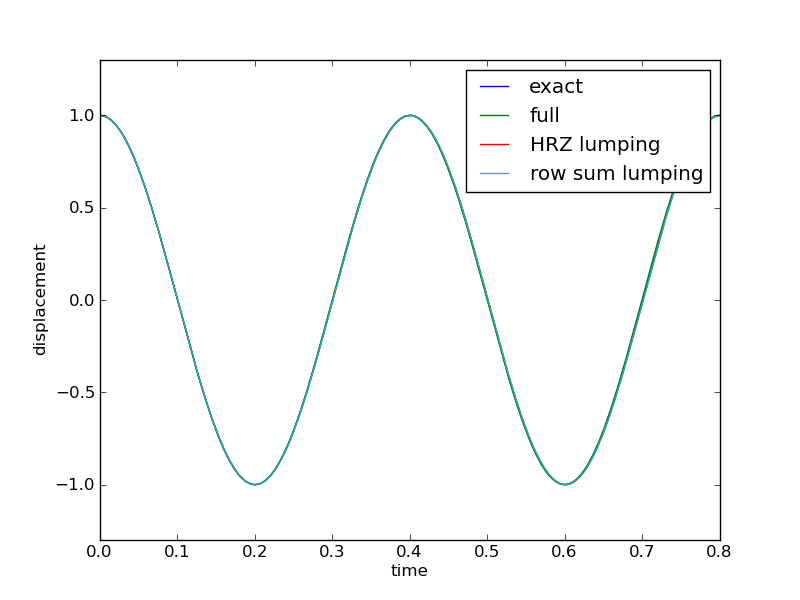
\includegraphics[width=7cm]{lumping_valet_a_1}}
\caption{Amplitude at point $(\frac{1}{2},\frac{1}{2})$ using the acceleration formulation~\ref{LUMPING WAVE VALET 2} of the 
Velet scheme with order $1$ elements, element size $dx=0.01$, and $c=1$.}
\label{FIG LUMPING VALET A}
\end{figure}

\begin{figure}[ht]
\centerline{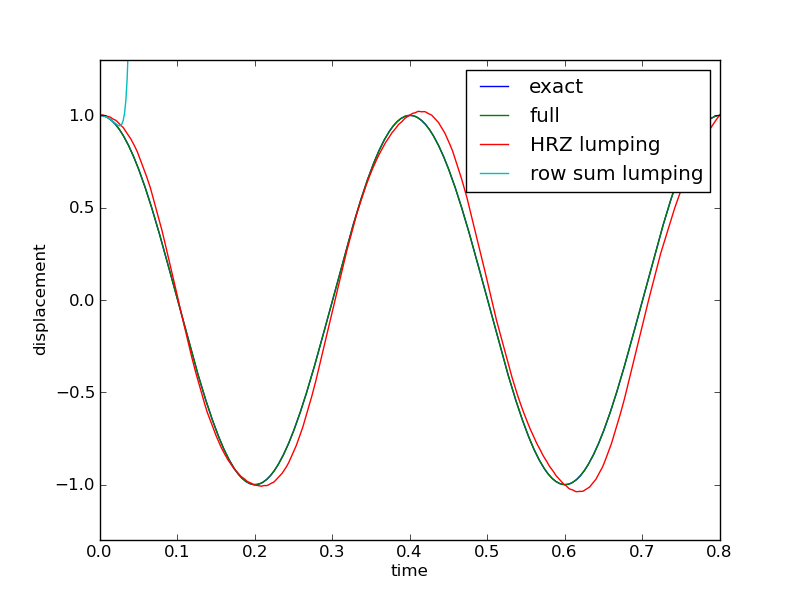
\includegraphics[width=7cm]{lumping_valet_a_2}}
\caption{Amplitude at point $(\frac{1}{2},\frac{1}{2})$ using the acceleration formulation~\ref{LUMPING WAVE VALET 2} of the 
Velet scheme with order $2$ elements, element size $0.01$, and $c=1$.}
\label{FIG LUMPING VALET B}
\end{figure}

\begin{figure}[ht]
\centerline{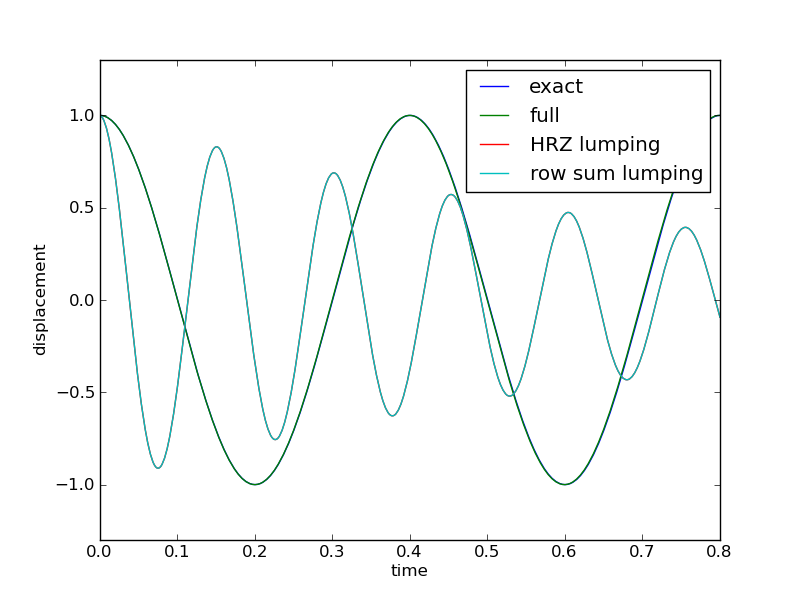
\includegraphics[width=7cm]{lumping_valet_u_1}}
\caption{Amplitude at point $(\frac{1}{2},\frac{1}{2})$ using the displacement formulation~\ref{LUMPING WAVE VALET 3} of the 
Velet scheme with order $1$ elements, element size $0.01$ and $c=1$.}
\label{FIG LUMPING VALET C}
\end{figure}

Alternatively, one can directly solve for $u^{(n)}$ by inserting 
equation~\ref{LUMPING WAVE VALET} into equation~\ref{LUMPING WAVE VALET 2}:
\begin{eqnarray} \label{LUMPING WAVE VALET 3} 
u^{(n)}=2u^{(n-1)}-u^{(n-2)} + (dt\cdot c)^2 u^{(n-1)}_{,ii} \; .
\end{eqnarray}
This can also be interpreted as a PDE that must be solved at each time-step, but 
for the unknown $u^{(n)}$. 
As per equation~\ref{LINEARPDE.SINGLE.1} we set the general form coefficients to:
$D=1$; $Y=2u^{(n-1)}-u^{(n-2)}$; and $X=-(h\cdot c)^2 u^{(n-1)}_{,i}$. 
For the full mass matrix, the acceleration ~\ref{LUMPING WAVE VALET 2} and displacement formulations ~\ref{LUMPING WAVE VALET 3}
are identical. 

The displacement solution is depicted in Figure~\ref{FIG LUMPING VALET C}. The
domain utilised order $1$ elements (for order $2$, both 
lumping methods are unstable). The solutions for the exact and the full mass 
matrix approximation are almost identical while the lumping solutions, whilst 
identical to each other, exhibit a considerably faster wave-front propagation 
and a decaying amplitude.

\subsection{Advection equation}
Consider now, a second example that demonstrates the advection equation
\begin{eqnarray} \label{LUMPING ADVECTIVE} 
u_{,t}=(v_i u)_i \; .
\end{eqnarray}
where $v_i$ is a given velocity field. To simplify this example, set $v_i=(1,0)$ and
\begin{equation} \label{LUMPING ADVECTIVE TEST} 
u(x,t)= 
\left\{
   \begin{array}{cl}
   1 &  x_0 < t \\
   0 &  x_0 \ge t 
   \end{array}
\right\}.
\end{equation}
The solution scheme implemented, is the two-step Taylor-Galerkin scheme 
\index{Taylor-Galerkin scheme}
(which is in this case equivalent to SUPG\index{SUPG}):
the incremental formulation is given as
\begin{eqnarray} \label{LUMPING SUPG 1} 
du^{(n-\frac{1}{2})} = \frac{dt}{2} (v_i u^{(n-1)})_i \\
du^{(n)} = dt (v_i (u^{(n-1)}+du^{(n-\frac{1}{2})}) )_i \\
u^{(n)} = u^{(n)} + du^{(n)} 
\end{eqnarray}
This can be reformulated to calculate $u^{(n)}$ directly:
\begin{eqnarray} \label{LUMPING SUPG 2} 
u^{(n-\frac{1}{2})} = u^{(n-1)} + \frac{dt}{2} (v_i u^{(n-1)})_i \\
u^{(n)} =  u^{(n-1)} + dt (v_i u^{(n-\frac{1}{2})} )_i 
\end{eqnarray}
In some cases it may be possible to combine the two equations to calculate 
$u^{(n)}$ without the intermediate step. This approach is not discussed, because
 it is inflexible when a greater number of terms (e.g. a diffusion term) are
 added to the right hand side. 

The advection problem is thus similar to the wave propagation problem, because 
the time step also needs to satisfy the CFL condition
\index{Courant condition}\index{explicit scheme!Courant condition}. For the 
advection problem, this takes the form
\begin{eqnarray} \label{LUMPING ADVECTION CFL} 
dt = f \cdot \frac{dx}{\|v\|} .
\end{eqnarray}
where $dx$ is the mesh size and $f$ is a safty factor. 
For this example, we again use $f=\frac{1}{6}$.

Figures~\ref{FIG LUMPING SUPG INC A} and~\ref{FIG LUMPING SUPG INC B} illustrate
the four incremental formulation solutions: the true solution; the exact mass matrix;
the HRZ lumping; and the row sum lumping. Observe, that for the order $1$ elements
case, there is little deviation from the exact solution before the wave front,
whilst there is a significant degree of osciallation after the wave-front has 
passed. For the order $2$ elements example, all of the numerical techniques fail. 

\begin{figure}[ht]
\centerline{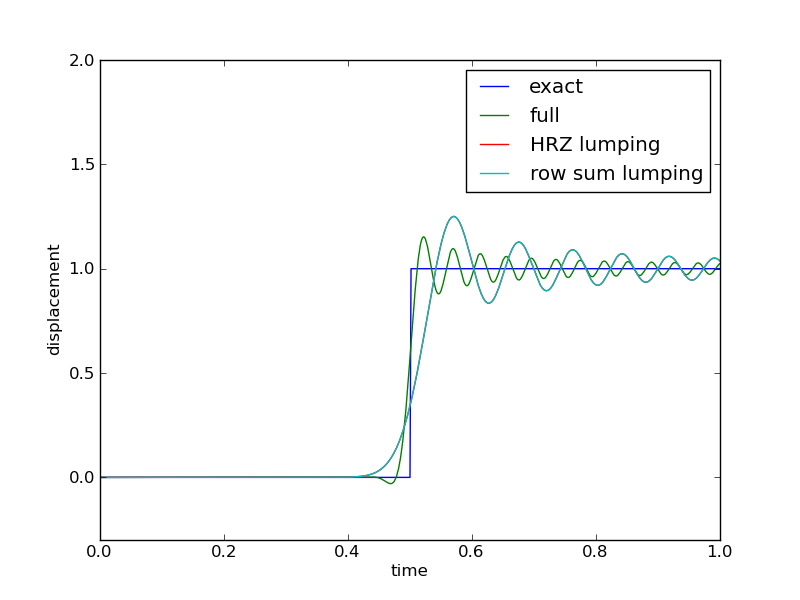
\includegraphics[width=7cm]{lumping_SUPG_du_1}}
\caption{Amplitude at point $(\frac{1}{2},\frac{1}{2})$ using the incremental formulation~\ref{LUMPING SUPG 1} of the 
Taylor-Galerkin scheme with order $1$ elements, element size $dx=0.01$, $v=(1,0)$.}
\label{FIG LUMPING SUPG INC A}
\end{figure}

\begin{figure}[ht]
\centerline{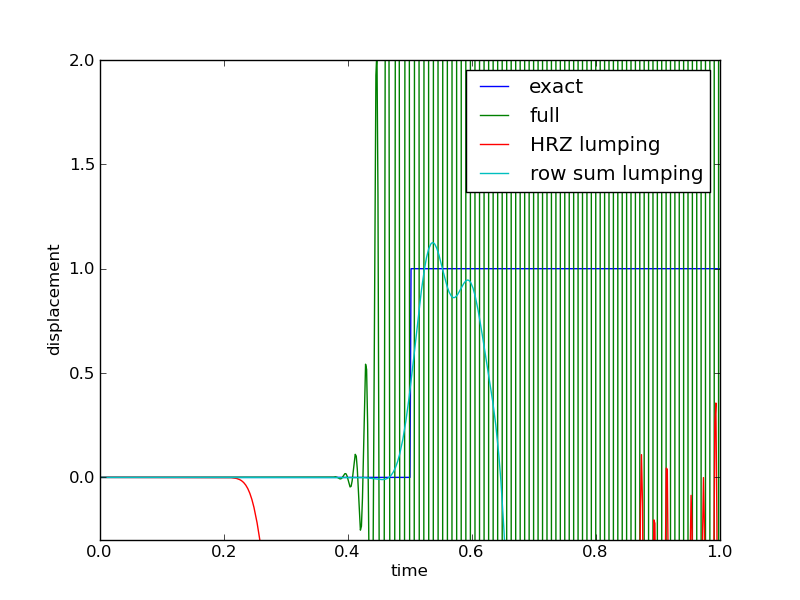
\includegraphics[width=7cm]{lumping_SUPG_du_2}}
\caption{Amplitude at point $(\frac{1}{2},\frac{1}{2})$ using the incremental formulation~\ref{LUMPING SUPG 1} of the 
Taylor-Galerkin scheme  with order $2$ elements, element size $0.01$, $v=(1,0)$.}
\label{FIG LUMPING SUPG INC B}
\end{figure}

Figure~\ref{FIG LUMPING SUPG A} depicts the results from the direct formulation
of the advection problem for an order $1$ mesh. Generally, the results have
improved when compared with the incremental formulation. The full mass matrix 
still introduces some osciallation both before and after the arrival of the 
wave-front at the observation point. The two lumping solutions are identical, and
have introduced additional smoothing to the solution. There are no oscillatory
effects when using lumping for this example. In Figure~\ref{FIG LUMPING SUPG Ab}
the mesh or element size has been reduced from 0.01 to 0.002 units. As predicted
by the CFL condition, this significantly improves the results when lumping is 
applied. However, when utilising the full mass matrix, a smaller mesh size will 
result in post wave-front oscilations which are higher frequency and slower to 
decay.

Figure~\ref{FIG LUMPING SUPG B} illustrates the results when utilising elements 
of order $2$. The full mass matrix and HRZ lumping formulations are unable to 
correctly model the exact solution. Only the row sum lumping was capable of 
producing a smooth and sensical result. 

\begin{figure}[ht]
\centerline{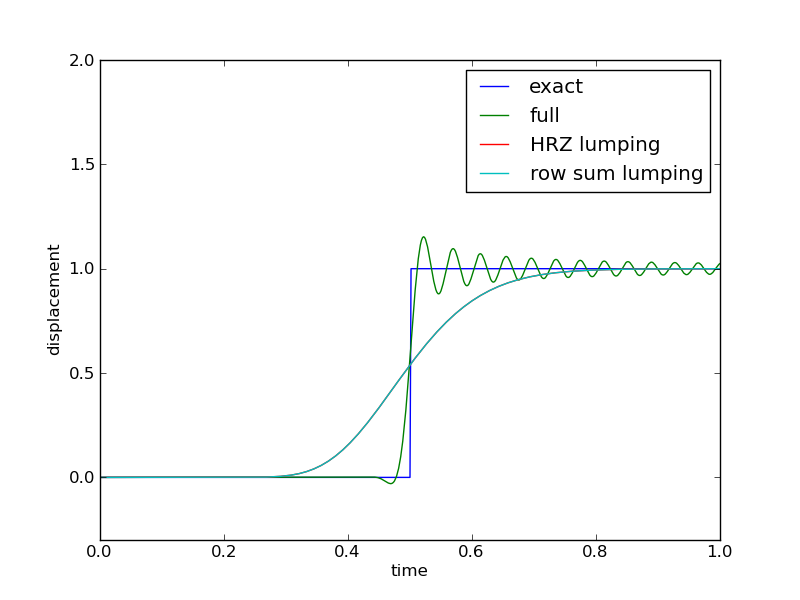
\includegraphics[width=7cm]{lumping_SUPG_u_1}}
\caption{Amplitude at point $(\frac{1}{2},\frac{1}{2})$ using the direct formulation~\ref{LUMPING SUPG 2} of the 
Taylor-Galerkin scheme using order $1$ elements, element size $dx=0.01$, $v=(1,0)$.}
\label{FIG LUMPING SUPG A}
\end{figure}

\begin{figure}[ht]
\centerline{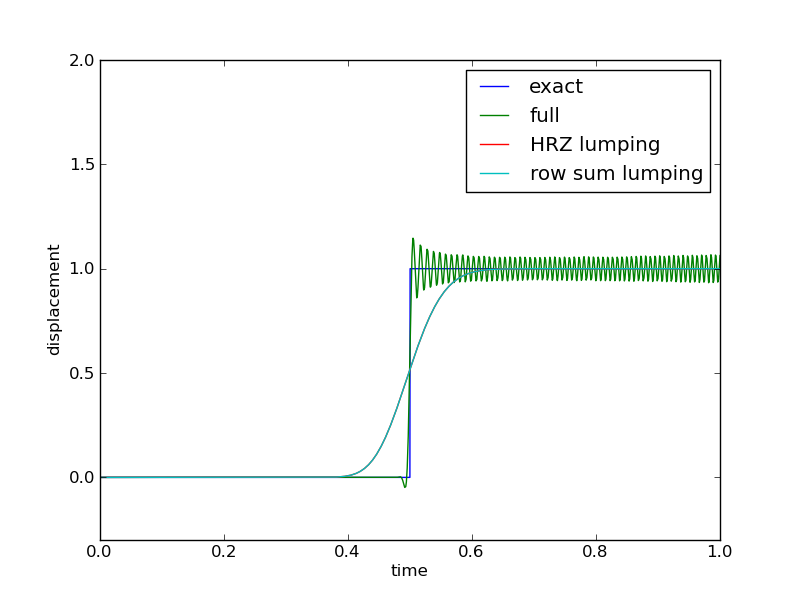
\includegraphics[width=7cm]{lumping_SUPG_u_1b}}
\caption{Amplitude at point $(\frac{1}{2},\frac{1}{2})$ using the direct formulation~\ref{LUMPING SUPG 2} of the 
Taylor-Galerkin scheme using order $1$ elements, element size $dx=0.002$, $v=(1,0)$.}
\label{FIG LUMPING SUPG Ab}
\end{figure}

\begin{figure}[ht]
\centerline{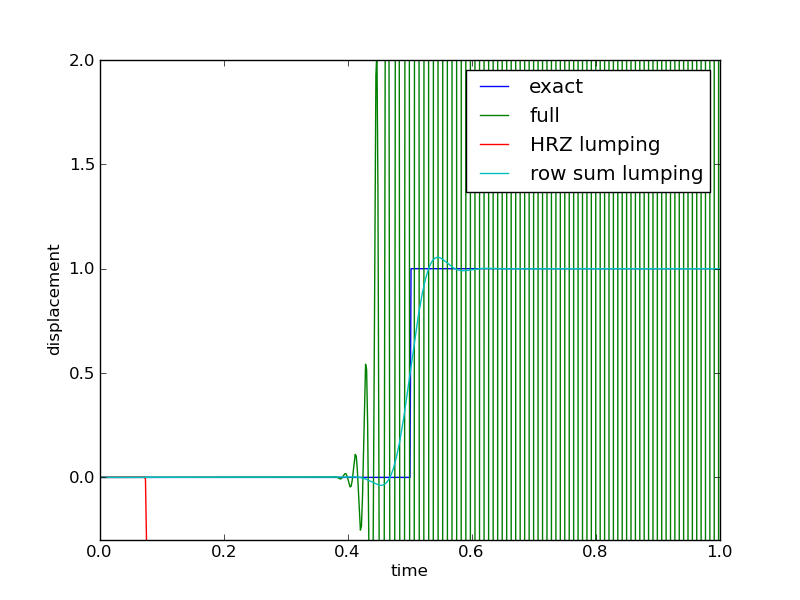
\includegraphics[width=7cm]{lumping_SUPG_u_2}}
\caption{Amplitude at point $(\frac{1}{2},\frac{1}{2})$ using the direct formulation~\ref{LUMPING SUPG 2} of the 
Taylor-Galerkin scheme  using order $2$ elements, element size $0.01$, $v=(1,0)$.}
\label{FIG LUMPING SUPG B}
\end{figure}

\subsection{Summary}
The examples in this section have demonstrated the capabilities and limitations
of both HRZ and row sum lumping with comparisons to the exact and full mass 
matrix solutions. Wave propagation type problems that utilise lumping, produce 
results simular the full mass matrix at significantly 
lower computation cost. An acceleration based formulation, with HRZ lumping 
should be implemented for such problems, and can be applied to both order $1$ and
 order $2$ elements. 

In transport type problems, it is essential that row sum lumping is used to 
achieve a smooth solution. Additionally, it is not recommended that second order
elements be used in advection type problems.




